\section{Enumeration-Based Synthesis Methodology\label{sec:ch6:enumeration}}

\begin{figure}
\centering
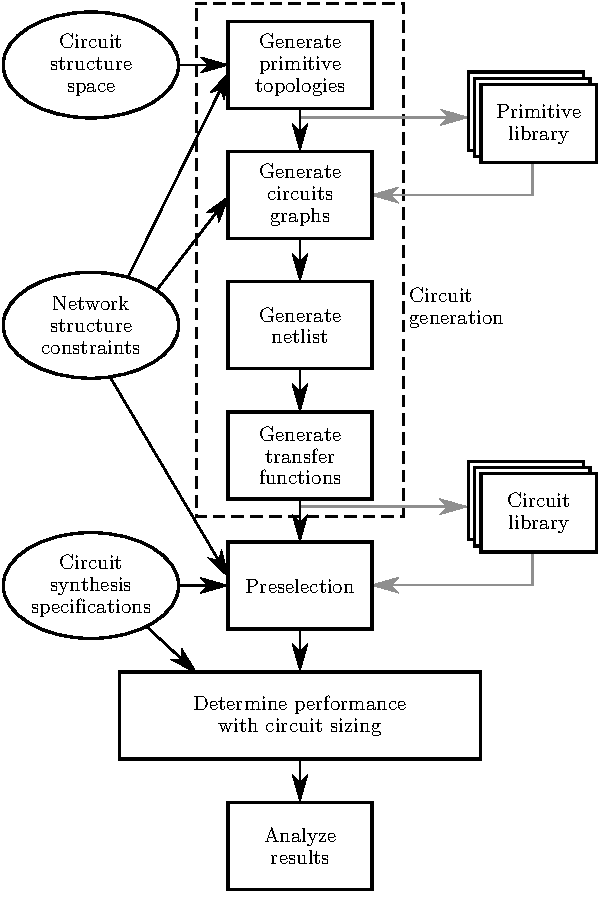
\includegraphics[width=0.6\textwidth]{../ch6/figures/algorithm.pdf}
\caption{Enumeration-based synthesis methodology.\label{fig:ch6:algorithm}}
\end{figure}

In this section, the procedure used to synthesize passive analog circuits is described. 
At the core of this approach is evaluating a set of circuits generated through an enumerative procedure. 
Figure~\ref{fig:ch6:algorithm} illustrates the overall flow of the enumeration-based synthesis framework.

\subsection{Representing Circuits as Colored Graphs}

\begin{figure}
\centering
\begin{subfigure}[b]{0.45\textwidth}
\centering
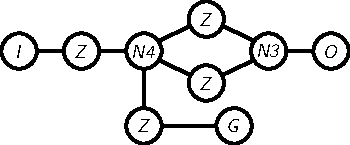
\includegraphics[scale=0.9]{../ch6/figures/steps_primitive}
\caption{Primitive circuit.\label{fig:ch6:steps:primitive}}
\end{subfigure}%
\hspace{0.05\columnwidth}%
\begin{subfigure}[b]{0.45\columnwidth}
\centering
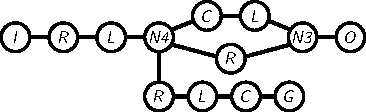
\includegraphics[scale=1.10]{../ch6/figures/steps_circuit}
\caption{Practical circuit.\label{fig:ch6:steps:circuit}}
\end{subfigure}%

\vspace{0.1in}

\begin{subfigure}[b]{0.4\textwidth}
\centering
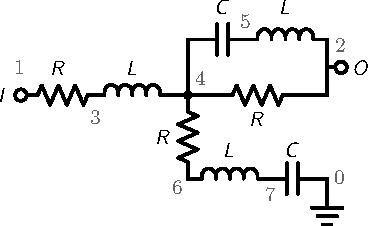
\includegraphics[width=0.9\textwidth]{../ch6/figures/steps_schematic}
\caption{Circuit schematic.}
\end{subfigure}%
\hspace{0.05\columnwidth}%
\begin{subfigure}[b]{0.4\textwidth}
\centering
\small
\begin{tabular}{c | c | c}
7 & 0 & \xcolor{C} \\
7 & 6 & \xcolor{L} \\
6 & 4 & \xcolor{R} \\
5 & 4 & \xcolor{C} \\
5 & 2 & \xcolor{L} \\
4 & 3 & \xcolor{L} \\
4 & 2 & \xcolor{R} \\
3 & 1 & \xcolor{R} \\
\end{tabular}
\caption{Netlist.\label{fig:ch6:netlist}}
\end{subfigure}
\caption{Different representations used for the same circuit.}
\end{figure}

Fundamental to this approach is the representation of circuits as colored graphs.
A colored (or labeled) graph is an extension of an undirected graph with an additional set defining the vertex or edge colors \cite{Gross2014a}.
Colored graphs in this chapter will always be vertex-colored graphs.
A properly defined colored graph will capture the topology of an electrical circuit.

% new paragraph
In a vertex-colored graph, circuit components such as resistors, capacitors, inductors, etc. can be represented as different vertex colors as is shown in Fig.~\ref{fig:ch6:steps:circuit}.
For example, every resistor in a circuit is labeled with $\xcolor{R}$ and is indistinguishable from one another.
If we are only concerned with the topology of the circuit network, not the specific components used, then we can use general impedance colors $\xcolor{Z}$ (see Fig.~\ref{fig:ch6:steps:primitive} for an example).
We will use the terms \textit{primitive circuit} if only general impedance elements are used and \textit{practical circuit} if specific components are present (such as the standard two-ports passive elements).
In this chapter, we will only consider two-port impedance elements, although the extension to multi-port impedance elements is possible.

% new paragraph
In addition to the impedance elements, additional voltage nodes in the circuit \cite{Ho1975a} will be labeled with $\xcolor{N}$. These are 0-junctions in bond graph modeling where the voltage is constant \cite{Borutzky2010a}.
Voltage nodes are further categorized by their number of connections (e.g.,~3-port voltage node vs. 4-port voltage node). Two $n$-port voltage nodes are then considered indistinguishable.
The distribution of voltage nodes in the circuit will vary (in Fig.~\ref{fig:ch6:steps:primitive}, there is one 3-port and one 4-port $\xcolor{N}$).
Similarly, the ground voltage node is labeled with $\xcolor{G}$.

% new paragraph
One advantage of a colored graph representation is colors can be used to represent a variety of concepts.
Many synthesis problems directly involve the input/output behavior of the synthesized circuit (e.g.,~\glsfirst{SISO} transfer function) \cite{Das2007a}.
We can use different colors to represent to location of the input and output nodes in the circuit (see Fig.~\ref{fig:ch6:steps:primitive} with colors $\xcolor{I}$ and $\xcolor{O}$).

% new paragraph
To summarize, circuits defined by colored graphs will contain colors representing two-port impedance elements, a variety of $n$-port voltage nodes, the ground node, the input node, and the output node.
With all relevant information included in the colored graphs, we can determine if two colored graphs are unique with respect to permutations of the vertices of the graphs \cite{Meissner2012a, Herber2017a}.
This is known as the colored graph isomorphism problem and is important to handle so that redundant circuits are not reused.

% new paragraph
There are other graph representations of circuits. 
A more common representation is an edge-colored graph with all vertices representing voltage nodes and edge colors representing different impedance types \cite{Gan2010a}.
Vertex coloring will be needed if the input and output nodes need to be identified.
The motivations behind the chosen representation is the ability to define intuitively the set of circuits that will be enumerated and leverage existing work in enumerating colored graphs \cite{Herber2017a}. These properties will become apparent in the following sections.

\subsection{Generating Primitive Circuits \label{sec:ch6:primitive}}

Enumeration of the primitive circuits is performed using a perfect matching-inspired algorithm where all ports of every component are connected to exactly one other port \cite{Herber2017a}.
In the worst case scenario, the growth of the number of graphs is $(N-1)!!$ where $N$ is the total number of ports and $\glsfirst{doublefac2}$ represents the double factorial function.
However, this bound is extremely conservative as many of the generated graphs are isomorphic (not unique) or do not satisfy \glsfirstplural[noindex]{NSC}.
Satisfaction of all NSCs defines the feasibility for a particular graph. 
Many enhancements to the original algorithm have been made in Ref.~\cite{Herber2017d}, further leveraging the structure of the enumeration task and allowing reasonably large graph structure spaces to be enumerated.
Here we will refer to the graph structure space covered by this approach as the circuit structure space\footnote{For more details on the enumeration approach used see Chapter~\ref{ch:2} and Appendix~\ref{app:A}.}.

% new paragraph
The required information for the enumeration approach is the following designer-defined elements:
\begin{itemize}
\item \gls{C} is the colored label sequence representing distinct component types
\item \gls{P} is a vector indicating the number of ports for each component type
\item $\gls{R}_{\glsfirst{min}}$ is a vector indicating the minimum number of replicates for each component type
\item $R_{\\glsfoo[noindex]{max}}$ is a vector indicating the maximum number of replicates for each component type
\end{itemize}

\noindent where we define $R$ as a matrix containing both $R_{\min}$ and $R_{\max}$.
For a circuit synthesis task, we could choose these elements as:
% 
\begin{subequations}
\label{eq:ch6:lib1}
\begin{gather}
C = \{ \xcolor{I}, \xcolor{O}, \xcolor{G}, \xcolor{Z}, \xcolor{N3}, \xcolor{N4}  \}, \quad P = \left[ 1\ 1\ 1\ 2\ 3\ 4 \right] \\
R_{\min} = \left[ 1\ 1\ 0\ 1\ 0\ 0 \right], \quad R_{\max} = \left[ 1\ 1\ 1\ 3\ 2\ 1 \right]
\end{gather}
\end{subequations}

\noindent where we have included the input node, output node, ground node, general two-port impedance elements, 3-port voltage nodes, and 4-port voltage nodes.
The input/output nodes and at least one impedance element are mandatory in any feasible graph.
In a feasible circuit, there can be up to three impedance elements, two 3-port voltage nodes, and one 4-port voltage node.
The choice of these elements is a major design decision and will be discussed further along with the examples presented in Sec.~\ref{sec:ch6:examples}.

% new paragraph
The addition of network structure constraints not only improves the quality of the generated graphs, but also decreases the computation time required for enumeration \cite{Herber2017a, Herber2017d}.
The first NSC is the requirement that every feasible graph has no loops or multi-edges. Next, we require that each graph is a connected graph so the input/output are guaranteed to be connected and there are no isolated components.

% new paragraph
The next set of NSCs limit the structure of the graph's adjacency matrix by ensuring zeros in certain locations:
\begin{itemize}
\item No ports from $\{ \xcolor{I}, \xcolor{O}, \xcolor{G} \}$ can be connected. If any of these are connected directly, then the transfer function for the circuit will be trivial and useless.

\item No ports from $\{ \xcolor{Z} \}$ can be connected. This would create series general impedance which is undesired during the generation of primitive circuits.

\item No ports from $\{ \xcolor{N3}, \xcolor{N4}, \cdots, \xcolor{N}x \}$ can be connected. This simply creates larger voltage nodes and we already restricted the maximum port size.
\end{itemize}

A final set of NSCs are some line-connectivity constraints \cite{Herber2017d}. Each constraint is specified as a triple of integers: [\#1,\#2,\#3] where each triple is interpreted as: if \#1 and \#2 are connected, don't ever connect \#2 to \#3.
For example, if we have $[1,5,2]$ and use Eqn.~(\ref{eq:ch6:lib1}), then we are enforcing if $\xcolor{I}$ is connected to $\xcolor{N3}$, then $\xcolor{N3}$ should not be connected to $\xcolor{O}$.
If we had $\xcolor{I} - \xcolor{N3} - \xcolor{O}$ present in a graph, the transfer function between the input and output would be unity.
To prevent such situations, we have that no voltage node ($\xcolor{N}x$) should be connected directly between any of the 1-port components $\{\xcolor{I}, \xcolor{O}, \xcolor{G} \}$.

% new pargraph
Based on these NSCs, we can filter out subcatalogs of $(C,P,R)$ that we know will not contain any feasible graphs; thus, reducing the computational expense when generating primitive circuits.
A subcatalog is a set of component replicates bounded by $(C,P,R)$ \cite{Herber2017d}.
Since no voltage node can be connected to another, their ports must be connected to the other component types. The same is true for $\{ \xcolor{I}, \xcolor{O}, \xcolor{G} \}$ and $\{ \xcolor{Z} \}$.
The 1-port components may be connected to either $\xcolor{Z}$ or $\xcolor{N}x$, resulting in two possible cases: one where all 1-port components are connected to $\xcolor{Z}$, and another only to $\xcolor{N}x$.
Then a necessary condition for a feasible graph to exist in a certain subcatalog under the NSCs is:
\begin{align} \label{eq:ch6:subcatalog:feas}
p_{\xcolor{N}} < p_{\xcolor{Z}} + \left( p_{\xcolor{I}} + p_{\xcolor{O}} + p_{\xcolor{G}} \right) \land p_{\xcolor{N}} > p_{\xcolor{Z}} - \left(p_{\xcolor{I}} + p_{\xcolor{O}} + p_{\xcolor{G}} \right)
\end{align}

\noindent where \gls{portsnum} indicates the total number of ports for component-type $x$ in the subcatalog.
For example for Eqn.~(\ref{eq:ch6:lib1}), the subcatalog $R_1=R_{\max}$ is infeasible due to the left condition ($10 \nless 9$), and the subcatalog $R_2=\left[ 1\ 1\ 0\ 3\ 1\ 0 \right]$ is infeasible due to the right condition ($3 \ngtr 4$).

% new paragraph
With the desired circuit structure space fully defined, we use enumeration to generate all possible unique graphs that satisfy the requirements above (see Ref.~\cite{github-pm-architectures-project} for the \textsc{Matlab} code for enumeration).
This set of graphs is termed the \textit{primitive library} and can be saved for future reuse.
For Eqn.~(\ref{eq:ch6:lib1}) with all the previously mentioned NSCs, there are 14 unique, feasible primitive graphs.
Each one of these primitive circuits is shown in Fig.~\ref{fig:ch6:primitive:lib}. Here we see many common topologies including parallel, series-parallel, L-section, and T-section.
\textit{All} topologies that can be constructed with respect to $(C,P,R)$ and the NSCs will be present.

\begin{figure}
\centering
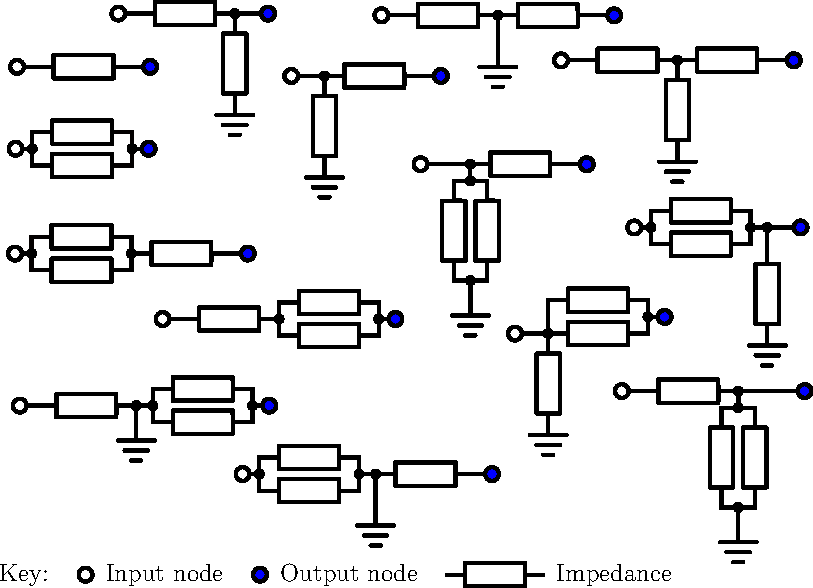
\includegraphics[width=0.55\columnwidth]{../ch6/figures/primitive_lib.pdf}
\caption{14 primitive circuits for the circuit structure space defined by Eqn.~(\ref{eq:ch6:lib1}).\label{fig:ch6:primitive:lib}}
\end{figure}

\subsection{Generating Practical Circuits}

For every primitive circuit in the primitive library, we want to transform the general impedance elements into practical components.
The designer must specify the potential subcircuits for these general impedance elements. Here we will consider subcircuits defined by series connections between $\{\xcolor{R}, \xcolor{L}, \xcolor{C}\}$ components, visualized in Fig.~\ref{fig:ch6:subcircuits}.
This set of subcircuits was chosen since the primitive graphs capture different ``parallel'' topologies and these subcircuits contain different ``series'' variations.

% new paragraph
It is important to understand the growth during this step so if there are $N$ potential subcircuits and $n$ general impedance components in the primitive circuit, then there are $(2^N - 1)^n$ practical circuits. If $N = 7$ and $n=4$, then there are 2,401 practical circuits for a single primitive circuit.
These permutations do not guarantee that each practical circuit is unique, so isomorphic checks must be performed.
Note that a practical circuit generated from primitive circuit $A$ will not be isomorphic to a practical circuit generated from primitive circuit $B$, so we only need to compare practical graphs from the same primitive circuit.
 
\begin{figure}
\centering
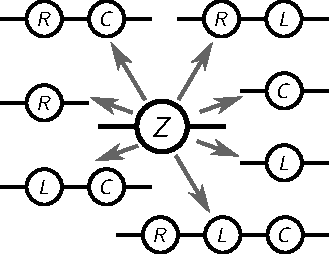
\includegraphics[width=0.3\columnwidth]{../ch6/figures/subcircuits.pdf}
\caption{Subcircuits considered for generating practical circuits (series \xcolor{RLC} subcircuits).\label{fig:ch6:subcircuits}}
\end{figure}

\subsection{Model Construction}

In many synthesis problems, there is a predefined \textit{template circuit} (or embryonic circuit) that contains some fixed circuit elements and their relation to the input node, output node, and ground \cite{Das2007a, Gan2010a, Goh2001a, Koza1997a, Lohn1999a}.
Two common template circuits are shown in Fig.~\ref{fig:ch6:template}.
A \textit{complete circuit} combines a practical circuit and the template circuit.

\begin{figure}[ht]
\centering
\begin{subfigure}[b]{0.4\textwidth}
\centering
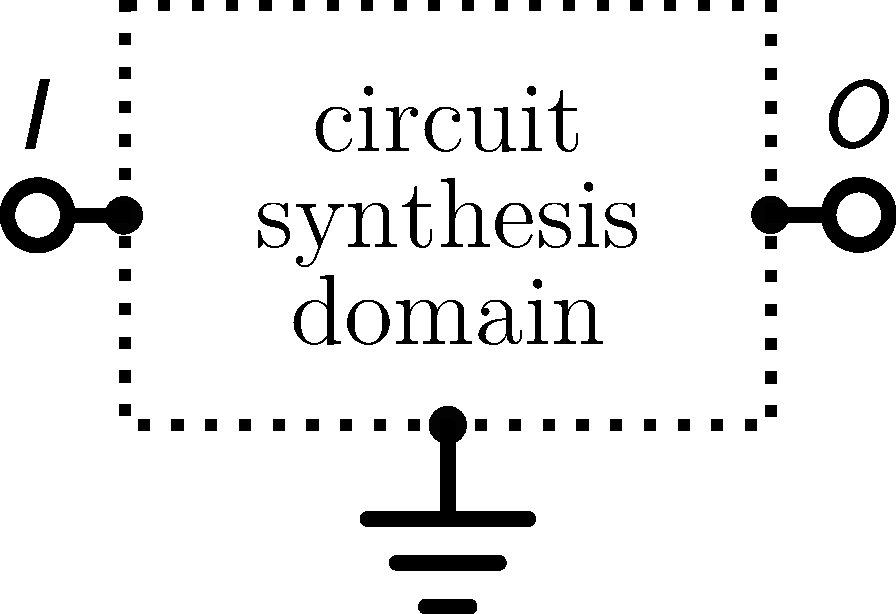
\includegraphics[scale = 0.20]{../ch6/figures/template_magnitude.pdf}
\caption{Frequency response.\label{fig:ch6:template:magnitude}}
\end{subfigure}%
\begin{subfigure}[b]{0.4\textwidth}
\centering
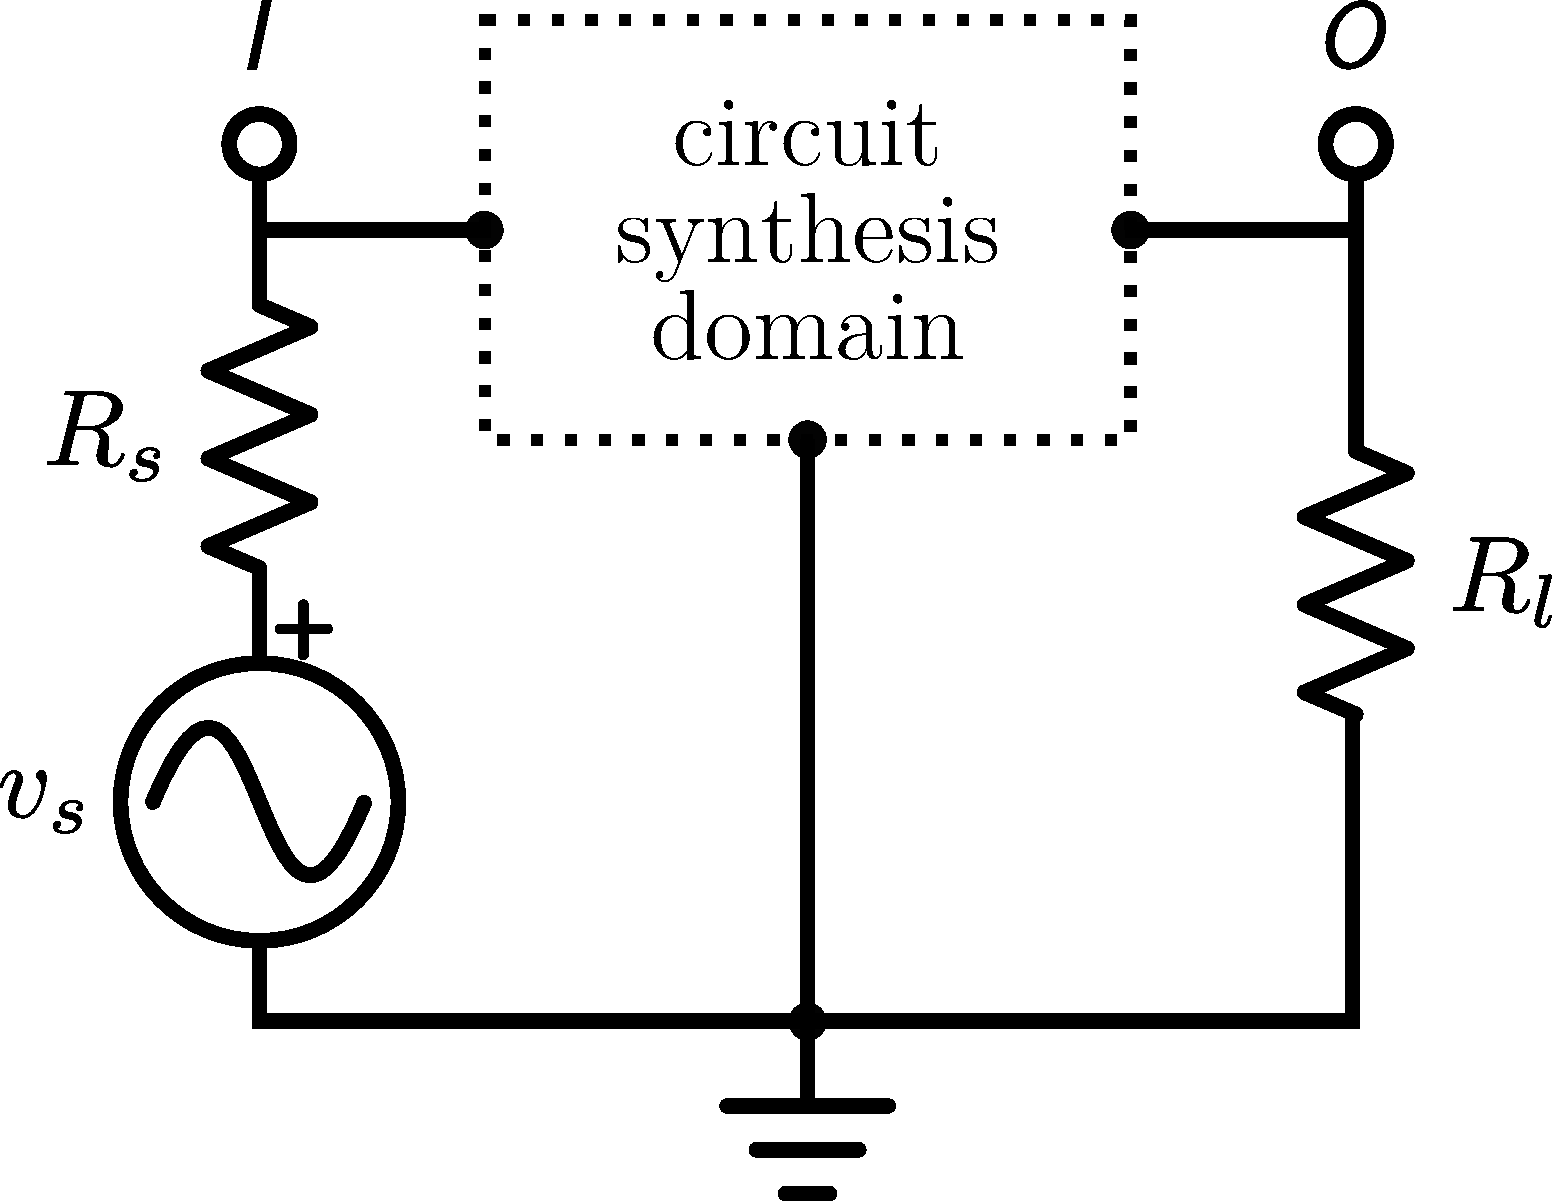
\includegraphics[scale = 0.20]{../ch6/figures/template_filter.pdf}
\caption{Filter.\label{fig:ch6:template:filter}}
\end{subfigure}%

\caption{Two common template circuits.\label{fig:ch6:template}}
\end{figure}

% new paragraph
For a complete circuit, a model is constructed by obtaining the transfer function between the input and output nodes, denoted \gls{G}.
This transfer function will depend on the frequency \gls{sfreq} and parameters from the template circuit \gls{rho} such as \gls{Rl} in Fig.~\ref{fig:ch6:template:filter}.
Additionally, optimization variables \gls{x} for the circuit are the coefficients for the two-port elements.
The distribution of the optimization variables will vary depending on the practical circuit.

% new paragraph
To generate $G(s, \bm{\rho}, \bm{x})$, we use \textsc{scam} \cite{scam}, a \textsc{Matlab} tool that derives and solves circuit equations symbolically using the modified nodal analysis method \cite{Ho1975a}.
This tool requires a netlist representation of the circuit, which is a set of triples that define the interconnections of circuit elements relative to numbered voltage nodes (see Fig.~\ref{fig:ch6:netlist} for an example).
It is fairly straightforward to generate the netlist from the colored graph representation.
The only exception is when voltage nodes are connected to any of the 1-port elements since these components are conceptually voltage nodes (and therefore are collapsed to a single voltage node). 

% new paragraph
The collection of all complete circuits and their models is termed the \textit{practical circuit library}, and can be saved for future reuse.
Using the primitive library in the previous section and the subcircuits from Fig.~\ref{fig:ch6:subcircuits}, there are 207 unique complete circuits.

\subsection{Preselection}

Preselection is an optional step that can be performed before the complete circuits are optimized for the particular synthesis task.
The designer can limit the circuits that are evaluated based on their preferences/constraints.
Some examples include:
\begin{itemize}
\item Bounds on the degrees of the polynomials $\gls{num}$ and $\gls{den}$, where $G(s) = N(s)/D(s)$

\item Bounds on the total number of components, \gls{nc}, sometimes considered a complexity measure \cite{Goh2001a}

\item Bounds on the distribution of the components (e.g.,~limit to a maximum of three resistors and two capacitors)

\item Bounds on the total number of circuits to evaluate, potentially selecting a fixed number of random circuits (although the coverage properties would no longer be present)

\end{itemize}

These preferences could be utilized to explore lower-complexity circuits first, checking whether higher complexity circuits are needed to satisfy the requirements of the synthesis task.
Since this approach uses a predefined library of circuits, these preferences/constraints can be handled readily.

\subsection{Evaluation}

With the desired set of complete circuits, we now need to determine how well the circuits satisfy a given synthesis problem.
Here we consider synthesis tasks that seek to minimize the error between desired transfer function properties and the circuit's physical response.
This involves sizing the circuit optimization variables $\bm{x}$.
Consider a set of $n_s$ frequency points, denoted \gls{freqset}, with desired values defined by $f(\gls{ofreq}_k)$.
Using a model function \glsfirst{model}, the synthesis task is posed as the following curving fitting problem:
\begin{subequations}
\label{eq:ch6:nls}
\begin{align}
\min_{\bm{x}} \quad & E = \sum \abs{r_k(\bm{x})}^2 \\
\text{subject to:} \quad & \bm{a}(\bm{x}) \leq \bm{0} \label{eq:ch6:add:constraints} \\
&\bm{l}  \leq \bm{x} \leq \bm{u} \label{eq:ch6:nls:bounds} \\
\text{where:} \quad & r_k = g(\omega_k,\bm{x}) - f(\omega_k) 
\end{align}
\end{subequations}

\noindent where \gls{error} is the error, \gls{residuals} are the individual residuals, \gls{ab} is the set of additional general constraints, and $\{\gls{lb},\gls{ub}\}$ are the lower and upper bounds on the optimization variables, respectively.
If there are no additional general constraints, then this is a standard \glsfirst{NLS} problem and suitable solvers are utilized \cite{matlab-lsqnonlin}.
Otherwise, general \glsfoo[noindex]{NLP} solvers will be used \cite{matlab-fmincon}.

% new paragraph
One suitable residual function for matching a circuit transfer function to a desired magnitude response is:
\begin{align}
\label{eq:ch6:rk:1}
r_k = \log\abs{G(\omega_k, \bm{x}) } - \log\abs{F(\omega_k) } = \log\abs*{\frac{G(\omega_k, \bm{x}) }{F(\omega_k) }}, \quad k = 1,\dots,n_s
\end{align}

\noindent i.e.,~we want to minimize the pointwise decibel error (ignoring the constant for simplicity since it does not effect the optimal curve fit).
Alternative residual functions have been suggested in the literature. Staying within the NLS framework, $r_k = G - F$ or $r_k = N - FD$ \cite{Levy1959a}.
Others utilized normalized versions \cite{Das2007a, Das2008a} or the sum of the absolute errors \cite{Goh2001a}.
The chosen function has been shown to produce solutions similar to the other residual functions but frequently is much smoother, improving convergence \cite{Arruda1992a}.

% new paragraph
Another useful residual function is when only feasibility is sought, i.e.,~find a suitable $\bm{x}$ such that Eqns.~(\ref{eq:ch6:add:constraints})--(\ref{eq:ch6:nls:bounds}) are satisfied.
This feasibility problem can be posed as a NLS using the following residual function:
\begin{align}\label{eq:ch6:res:feas}
r_k = \max\big(0, a_k( \bm{x}) \big), \quad k = 1,\dots,n_a
\end{align}

\noindent where \gls{na} is the number of constraints. This results in a common penalty method used with NLP \cite{Chinneck2008a}. % page 52

% new paragraph
Some studies also introduce heuristic penalty functions to help penalize higher-complexity circuits \cite{Grimbleby1995a, Grimbleby2000a}.
Complexity penalization is not needed in the optimization formulation as it can be readily computed offline because the distribution of circuit elements is not changing, as is the case in an evolutionary approach.

% new paragraph
Two other aspects of the evaluation procedure are a possible weight function and linear frequency scaling.
A weight function may be defined as $E = \sum w(\omega_k) \abs{r_k(\bm{x})}^2$ where \gls{weights} is the weight function that may be used to give less attention to high frequencies, provide greater weight to specific regions of interest, or combine multiobjectives \cite{Das2007a, Das2008a}.
We will also use simple linear scaling of the frequency, i.e.,~$s = \gls{alpha} \bar{s}$ where $\alpha > 0$.
This is done for numerical stability reasons and we will use the following recommendation from Ref.~\cite{Pintelon1994a}:
$\alpha = \big(\min(\Omega) + \max(\Omega)\big)/2$.

% new paragraph
Due to the complexity of the proposed nonlinear program, it may be challenging to find a feasible solution or solutions near the global optimum. 
To help remedy this issue, a multi-start approach is utilized \cite{Marti2003a}.
Here a large number of stratified random samples (100,000) were initially tested and the best five were used as initial points in independent optimization runs.

% new paragraph
When the performance of all the circuits has been evaluated, the results can be analyzed.
Unlike other synthesis approaches, there are potentially a large number of feasible circuits to choose from.
Having many alternatives is a significant advantage.
Tradeoffs in complexity vs. performance can readily be observed. For example, we can find the lowest complexity feasible circuit.
Alternatively, if no feasible circuits are found, we have gained some insights into the types of circuits that will be required to satisfy the synthesis task.
These post-processing analysis tasks will be discussed more in the \nameref{sec:ch6:discussion} section.